% The document class supplies options to control rendering of some standard
% features in the result.  The goal is for uniform style, so some attention 
% to detail is *vital* with all fields.  Each field (i.e., text inside the
% curly braces below, so the MEng text inside {MEng} for instance) should 
% take into account the following:
%
% - author name       should be formatted as "FirstName LastName"
%   (not "Initial LastName" for example),
% - supervisor name   should be formatted as "Title FirstName LastName"
%   (where Title is "Dr." or "Prof." for example),
% - degree programme  should be "BSc", "MEng", "MSci", "MSc" or "PhD",
% - dissertation title should be correctly capitalised (plus you can have
%   an optional sub-title if appropriate, or leave this field blank),
% - dissertation type should be formatted as one of the following:
%   * for the MEng degree programme either "enterprise" or "research" to
%     reflect the stream,
%   * for the MSc  degree programme "$X/Y/Z$" for a project deemed to be
%     X%, Y% and Z% of type I, II and III.
% - year              should be formatted as a 4-digit year of submission
%   (so 2014 rather than the academic year, say 2013/14 say).

\documentclass[ % the name of the author
                    author={Lucas O'Dowd-Jones},
                % the name of the supervisor
                supervisor={Dr. Alex Kavvos},
                % the degree programme
                    degree={MEng},
                % the dissertation    title (which cannot be blank)
                     title={Variations on Normalisation by Evaluation in Haskell},
                % the dissertation subtitle (which can    be blank)
                  subtitle={},
                % the dissertation     type
                      type={programming languages},
                % the year of submission
                      year={2021} ]{dissertation}

\usepackage{amsmath}
\usepackage{biblatex}
\addbibresource{bibliography.bib}
\usepackage{listings}
\lstset{
  basicstyle=\ttfamily\small,
  keywordstyle=[0]\bfseries\color{bittersweet},
  keywordstyle=[1]\bfseries\color{teal},
  keywordstyle=[2]\bfseries,
  columns=spaceflexible,
  morekeywords=[0]{data, where, type, class, instance},
  morekeywords=[1]{Nat, List, Sorted, Uniq, Eq, Ty, BaseTy},
  morekeywords=[2]{Z, S, True},
  mathescape=true,
  keepspaces=true,
  aboveskip=10pt,
  belowskip=10pt
}

\begin{document}
\definecolor{teal}{rgb}{0.0, 0.5, 0.5}
\definecolor{bittersweet}{rgb}{1.0, 0.44, 0.37}

% =============================================================================

% This macro creates the standard UoB title page by using information drawn
% from the document class (meaning it is vital you select the correct degree 
% title and so on).

\maketitle

% After the title page (which is a special case in that it is not numbered)
% comes the front matter or preliminaries; this macro signals the start of
% such content, meaning the pages are numbered with Roman numerals.

\frontmatter

% This macro creates the standard UoB declaration; on the printed hard-copy,
% this must be physically signed by the author in the space indicated.

\makedecl

% LaTeX automatically generates a table of contents, plus associated lists 
% of figures, tables and algorithms.  The former is a compulsory part of the
% dissertation, but if you do not require the latter they can be suppressed
% by simply commenting out the associated macro.

\tableofcontents
\listoffigures
\listoftables
\listofalgorithms
\lstlistoflistings

% The following sections are part of the front matter, but are not generated
% automatically by LaTeX; the use of \chapter* means they are not numbered.

% -----------------------------------------------------------------------------

\chapter*{Executive Summary}

% {\bf A compulsory section, of at most $1$ page} 

\noindent
This section should pr\'{e}cis the project context, aims and objectives,
and main contributions (e.g., deliverables) and achievements; the same 
section may be called an abstract elsewhere.  The goal is to ensure the 
reader is clear about what the topic is, what you have done within this 
topic, {\em and} what your view of the outcome is.

The former aspects should be guided by your specification: essentially 
this section is a (very) short version of what is typically the first 
chapter.  Note that for research-type projects, this {\bf must} include 
a clear research hypothesis.  This will obviously differ significantly
for each project, but an example might be as follows:

\begin{quote}
My research hypothesis is that a suitable genetic algorithm will yield
more accurate results (when applied to the standard ACME data set) than 
the algorithm proposed by Jones and Smith, while also executing in less
time.
\end{quote}

\noindent
The latter aspects should (ideally) be presented as a concise, factual 
bullet point list.  Again the points will differ for each project, but 
an might be as follows:

\begin{quote}
\noindent
\begin{itemize}
\item I spent $120$ hours collecting material on and learning about the 
      Java garbage-collection sub-system. 
\item I wrote a total of $5000$ lines of source code, comprising a Linux 
      device driver for a robot (in C) and a GUI (in Java) that is 
      used to control it.
\item I designed a new algorithm for computing the non-linear mapping 
      from A-space to B-space using a genetic algorithm, see page $17$.
\item I implemented a version of the algorithm proposed by Jones and 
      Smith in [6], see page $12$, corrected a mistake in it, and 
      compared the results with several alternatives.
\end{itemize}
\end{quote}

% -----------------------------------------------------------------------------

\chapter*{Supporting Technologies}

% {\bf A compulsory section, of at most $1$ page}

\noindent
This section should present a detailed summary, in bullet point form, 
of any third-party resources (e.g., hardware and software components) 
used during the project.  Use of such resources is always perfectly 
acceptable: the goal of this section is simply to be clear about how
and where they are used, so that a clear assessment of your work can
result.  The content can focus on the project topic itself (rather,
for example, than including ``I used \mbox{\LaTeX} to prepare my 
dissertation''); an example is as follows:

\begin{quote}
\noindent
\begin{itemize}
\item I used the Java {\tt BigInteger} class to support my implementation 
      of RSA.
\item I used a parts of the OpenCV computer vision library to capture 
      images from a camera, and for various standard operations (e.g., 
      threshold, edge detection).
\item I used an FPGA device supplied by the Department, and altered it 
      to support an open-source UART core obtained from 
      \url{http://opencores.org/}.
\item The web-interface component of my system was implemented by 
      extending the open-source WordPress software available from
      \url{http://wordpress.org/}.
\end{itemize}
\end{quote}

% -----------------------------------------------------------------------------

\chapter*{Notation and Acronyms}

% {\bf An optional section, of roughly $1$ or $2$ pages}

\noindent
Any well written document will introduce notation and acronyms before
their use, {\em even if} they are standard in some way: this ensures 
any reader can understand the resulting self-contained content.  

Said introduction can exist within the dissertation itself, wherever 
that is appropriate.  For an acronym, this is typically achieved at 
the first point of use via ``Advanced Encryption Standard (AES)'' or 
similar, noting the capitalisation of relevant letters.  However, it 
can be useful to include an additional, dedicated list at the start 
of the dissertation; the advantage of doing so is that you cannot 
mistakenly use an acronym before defining it.  A limited example is 
as follows:

\begin{quote}
\noindent
\begin{tabular}{lcl}
AES                 &:     & Advanced Encryption Standard                                         \\
DES                 &:     & Data Encryption Standard                                             \\
                    &\vdots&                                                                      \\
${\mathcal H}( x )$ &:     & the Hamming weight of $x$                                            \\
${\mathbb  F}_q$    &:     & a finite field with $q$ elements                                     \\
$x_i$               &:     & the $i$-th bit of some binary sequence $x$, st. $x_i \in \{ 0, 1 \}$ \\
\end{tabular}
\end{quote}

% -----------------------------------------------------------------------------

\chapter*{Acknowledgements}

% {\bf An optional section, of at most $1$ page}

\noindent
It is common practice (although totally optional) to acknowledge any
third-party advice, contribution or influence you have found useful
during your work.  Examples include support from friends or family, 
the input of your Supervisor and/or Advisor, external organisations 
or persons who  have supplied resources of some kind (e.g., funding, 
advice or time), and so on.

% =============================================================================

% After the front matter comes a number of chapters; under each chapter,
% sections, subsections and even subsubsections are permissible.  The
% pages in this part are numbered with Arabic numerals.  Note that:
%
% - A reference point can be marked using \label{XXX}, and then later
%   referred to via \ref{XXX}; for example Chapter\ref{chap:context}.
% - The chapters are presented here in one file; this can become hard
%   to manage.  An alternative is to save the content in seprate files
%   the use \input{XXX} to import it, which acts like the #include
%   directive in C.

\mainmatter

% -----------------------------------------------------------------------------

\chapter{Introduction}
\label{chap:introduction}

% Start with want to implement functional language
To implement a functional programming language, we need a normalisation function that maps each expression in the functional language to its normal form.
% We use NbE
In this dissertation we explore various implementations of Normalisation by Evaluation (NbE) for the lambda calculus.

% What/how it works roughly
NbE proceeds by interpreting terms of the lambda calculus (referred to as “syntax”) as elements of a mathematical “semantic” set. NbE then “reifies” semantic values back into the set of normal terms. All $\beta$-equal terms “evaluate” to the same semantic value, so $\beta$-equal terms normalise to the same normal form.

% Why do we care
    % Modern
NbE is a modern alternative to normalisation by reduction; a technique based on syntactic rewriting. NbE is useful for the following reasons.

\begin{enumerate}
    \item Since the foundations of NbE are mathematical, we can prove that our implementation is correct and study its behaviour formally \cite{AgdaNbe}. Proving that the implementations are fully correct is beyond the scope of this project, but we use types as machine-checked proof that our implementation satisfies certain properties.
    \item Some research suggests that NbE can improve the speed of compilation of functional languages \cite{efficientNbE}.
    \item Research is ongoing into whether dependent type theories such as Coq can use NbE to check for equality between dependent types by normalising type-level programs \cite{deBruijn}
\end{enumerate}

% --roadmap
To become familiar with the general operation of NbE, in Chapter \ref{chap:untypednbe} we present two implementations for NbE of the untyped lambda calculus. The first implementation normalises the named lambda calculus. This implementation works, but its correctness depends on fresh name generation which makes it difficult to reason about. This issue motivates a second implementation of NbE, where we normalise a nameless representation of the lambda terms instead. Since variable names are not part of this syntax, fresh variables are much easier to generate.

Then we move to the central challenge of this project: translating an Agda implementation of NbE for the Simply Typed Lambda Calculus (STLC) into Haskell. The Agda implementation we follow makes use of advanced type-level features such as dependent types and dependent pattern matching. However, Agda is currently unsuitable for general-purpose programming for the following reasons

\begin{enumerate}
    \item It is a type theory and proof assistant primarily, rather than a general-purpose programming language
    \item It has a steep learning curve due to the theoretical understanding required to develop programs
    \item The community supporting it is small and mainly academic
\end{enumerate}

Haskell is a mature language suitable for industry use \cite{haskellInIndustry} as it strikes a balance between theory and practice, allowing developers to take advantage of type-safety without as much theoretical overhead. However, recent compiler options have enabled the use of advanced type-features more akin to dependently typed languages such as Agda. 

Through implementing NbE for the STLC, this project will assess whether Haskell can be used to emulate features of languages with full dependent types. Members of the Haskell community are actively working on bringing full dependent types to Haskell \cite{DH}, but this project serves as an evaluation of how well the existing tooling for complex types works in practice.

In Chapter \ref{chap:typedlamadacalculus}, we use introduce and use Generalised Algebraic Datatypes (GADTs) in conjunction with the \code{DataKinds} and \code{PolyKinds} extensions to define terms that are well-typed by construction. 
In Chapter \ref{chap:typednbe} we implement the well-typed normalisation function. For this we need the \code{RankNTypes} extension, which gives finer control over quantification in polymorphic type signatures, and \code{ScopedTypeVariables}, to bind type variables within function bodies. To emulate reflection of dependent types from the type level to the value level at runtime, we explore a method inspired by the singleton pattern \cite{singletons}.

The aims of this project are:
\begin{enumerate}
    \item To produce various implementations of NbE in Haskell
    \item To explore how successful modern features of Haskell are in implementing an algorithm with complex types.
\end{enumerate}

% -----------------------------------------------------------------------------

\chapter{Normalising the Untyped Lambda Calculus}
\label{chap:untypednbe}

\section{Overview of the NbE algorithm}

\begin{figure}[h]
    \centering
    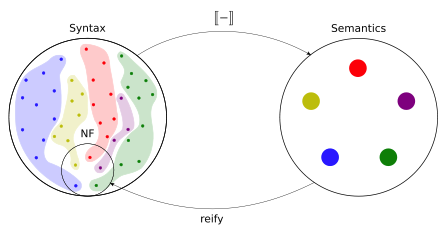
\includegraphics[width=0.6\textwidth]{./images/nbe_diagram}
    \caption{A visual overview of the NbE algorithm from \cite{slides}}
    \label{fig:nbeOverview}
\end{figure}

NbE proceeds in two steps. The first is to evaluate terms in the lambda calculus into a semantic set. In \ref{fig:nbeOverview} terms are represented by dots in the syntax set and the evaluation function is denoted by $\llbracket - \rrbracket$, which we refer to as \code{eval}. The second step is to \code{reify} the semantic value back into the normal form of the original term. Thus, the \code{normalise} function which maps terms to their normal forms is the composition of \code{eval} and \code{reify}

% property of eval
\ref{fig:nbeOverview} illustrates why NbE works. The key property of the \code{eval} function is that $\beta$-equal terms (represented by dots of the same colour in the syntax set) evaluate to the same semantic value. This ensures that $\beta$-equal terms normalise to the same normal form. The key property of the \code{reify} function is that the codomain of \code{reify} is the subset of normal forms, so \code{normalise} is guaranteed to return a normal form. 

The remainder of this chapter defines the data NbE operates on and functions to perform NbE in Haskell.

\section{Syntax}

\begin{lstlisting}
    type Name = String

    data Expr = ExpVar Name
              | ExpLam Name Expr
              | ExpApp Expr Expr
\end{lstlisting}

Inhabitants of the inductively-defined datatype \code{Expr} are well-formed terms of the untyped lambda calculus with strings as variables. The first argument of the lambda case introduces a new variable name bound in the function body defined by the second argument. For example, the identity function $\lambda x . x$ would be encoded as \code{ExpLam "x" (ExpVar "x")}.

\begin{lstlisting}
    data NormalForm = NfNeutralForm NeutralForm
                    | NfLam Name NormalForm

    data NeutralForm = NeVar Name
                     | NeApp NeutralForm NormalForm
\end{lstlisting}

We now define the target syntax of the \code{normalise} function, \code{NormalForm}. Note that \code{NormalForm} is inhabited by all the terms not containing $\beta$-redexes \cite{slides}, since the definition of \code{NeApp} only permits application on non-lambda terms, which are encoded as values of type \code{NeutralForm}.

\section{Semantics}

\begin{lstlisting}
    data V = Neutral NeutralV
           | Function (V -> V)

    data NeutralV = NeVVar Name
                  | NeVApp NeutralV V
\end{lstlisting}

% TODO: Mentional easy to define V -> V in Haskell, harder in other languages, motivating advantage of Haskell?

The semantic set \code{V} has a very similar structure to the set of normal forms, however lambda terms are replaced with Haskell functions of type \code{V} $\rightarrow$ \code{V}.
% TODO: Include following paragraph or not - not justified? 
The similarity simplifies \code{reify} as for some terms there are obvious translations from semantics to syntax. The replacement of lambda terms will be useful in evaluating $\beta$-redexes at the semantic level instead of the syntactic level. 

% TODO: Discuss using why don't use Neutral Form but establish our own datatype

\section{Evaluation}

Evaluation proceeds by pattern matching on the given term, and evaluating its constituent subterms. However, the semantic meaning of subterms can differ depending on which variables are bound by which lambda term. For example, in the terms $\lambda x . \lambda y . xy$ and $\lambda y . xy$, the semantic meaning of the $xy$ subterm is different. Thus, in addition to the term itself, \code{eval} needs information about the bound variables introduced by surrounding lambda terms. 

To keep track of which variables have been bound by surrounding lambda terms, we construct an environment datatype.

\begin{lstlisting}
    type Env = Map Name V
\end{lstlisting}

Each key of the map corresponds to a bound variable name, and its associated value is the semantic value representing the variable. The environment can be thought of as the scope each subterm is evaluated in. 
% TODO: Include or not - helpful or overly general waffle?
It expands as more variables are bound in deeper subterms.

\begin{lstlisting}
    eval :: Expr -> Env -> V
\end{lstlisting}

\code{eval} takes an expression and the environment to evaluate it in, pattern matches on the expression, and returns the interpretation of the term in the semantic set. We now discuss the implementation of each case of the pattern match.

\begin{lstlisting}
    eval (ExpVar x) env = case lookup x env of
        Just y -> y
        Nothing -> Neutral (NeVVar x)
\end{lstlisting}

In the variable case, we lookup the variable in the environment. If the variable was bound by a surrounding lambda term, the variable will be present in the environment, and we can return the semantic value associated with it. Otherwise, the variables is free, so we return a semantic variable with the same name.

\begin{lstlisting}
    eval (ExpLam var m) env = Function f where
        f :: V -> V
        f v = eval m env' where
            env' = insert var v env
\end{lstlisting}

% TODO: Include or not, repeating code in words?
The semantic interpretation of a lambda expression is a Haskell function of type \code{V} $\rightarrow$ \code{V}. This function takes an element \code{v} of the semantic set \code{V}, and returns the body of the lambda evaluated in an extended environment \code{env'}. In this extended environment, we bind the named variable \code{var} to \code{v}.

From the variable case, we see that whenever the variable \code{ExpVar var} is evaluated in the function body it will be interpreted as \code{v}. We can think of \code{v} as a semantic placeholder for the value \code{f} is applied to (if any). The use of this approach is demonstrated in the application case.

\begin{lstlisting}
    eval (ExpApp m n) env = app (eval m env) (eval n env)
        where
            app :: V -> V -> V
            app (Function f) v0 = f v0
            app (Neutral n)  v0 = Neutral (NeVApp n v0)
\end{lstlisting}

In the application case we evaluate the \code{m} and \code{n} terms in the same environment, before applying them to \code{app}, which handles the application of semantic values. 

In the case where the first value is a function \code{f}, we evaluate \code{f} at the second argument \code{v0}. From the lambda case we see that this subcase corresponds to evaluating a redex term. Instead of contracting the redex by substituting at the syntactic level, we evaluate it using function application at the semantic level. The application instantiates the placeholder \code{v} at the semantic value \code{v0} in the lambda body. 

% TODO: Explain more
In the case that the first value is a value \code{n} of type \code{NeutralV}, there is no redex to contract, so we return a placeholder Neutral application at the semantic level.

\section{Gensym Reification}

% TODO: Cite name, in de Bruijn paper

Reification proceeds by pattern matching on the semantic value, and recursively reifying its constituent values.

Since evaluating a lambda yields a function, reifying a function should yield a lambda to ensure that \code{normalise} preserves terms already in normal form. But what variable should the returned lambda term bind? The new bound variable should be different to all other bound variables in scope, otherwise \code{reify} could produce invalid terms. It should also be different to all other free variables in the original term, to prevent free variable capture. Since terms are considered equal up to bound variable renaming by $\alpha$-equivalence, we can choose any variable name that satisfies these requirements. 

One approach to resolve this issue suggested by \cite{slides} is to generate a fresh variable name during reification whenever a new bound variable is needed. However, generating fresh variables during the execution of \code{reify} would require the function to track which variables have already been bound between calls to \code{reify}, which suggests the use of state. This could be modelled using the \code{State} monad, in which case \code{reify} would have the type signature \code{reify :: V -> State [Name] NormalForm}, where \code{[Name]} corresponds to a list of variable names that have already been bound. This would allow us to implicitly pass the list of bound variable names between calls to reify. However state introduces additional complexity and makes testing more difficult, which can lead to flawed implementations.

%TODO: other problems with state monad (not really used mostly passing => redundant boilderplate to carry monad round), link to State monad implementation

Instead, we opt for a more functional approach. Before the execution of \code{reify}, we generate a suitable stream of fresh variable names of type \code{[Name]}. By making \code{reify} a function of the semantic element and the stream of fresh variables, we can simply pop a fresh variable name from the stream whenever a new variable is bound. In recursive calls, \code{reify} only passes the tail of the stream to ensure bound variable names are never reused.

\begin{lstlisting}
    reify :: V -> [Name] -> NormalForm
\end{lstlisting}

\code{reify} proceeds by pattern matching on the first argument of type \code{V}. 

\begin{lstlisting}
    reify (Neutral n)  freshVars = NfNeutralForm (reifyNeutral n freshVars)

    reifyNeutral :: NeutralV -> [Name] -> NeutralForm
    reifyNeutral (NeVVar i)   freshVars = NeVar i
    reifyNeutral (NeVApp n m) freshVars = NeApp reifiedN reifiedM
        where
            reifiedN = reifyNeutral n freshVars
            reifiedM = reify m freshVars
\end{lstlisting}

In the neutral case, we use \code{reifyNeutral} to convert the value \code{n} of type \code{NeutralV} to a \code{NeutralForm}, which is promoted to a \code{NormalForm} by the \code{NfNeutralForm} constructor. The \code{reifyNeutral} function also proceeds by patten matching. 

In the variable case we extract a neutral syntactic variable of the same name as the semantic variable. 

In the application case we reify the semantic values \code{n} and \code{m}, and return a neutral syntactic application of the resulting terms.
% TODO: Check this - talk about independece between reifyiedN and reifiedM, reword
We are able to reify both semantic values using the same fresh variable stream since the returned value is a \code{NeutralForm}, which by definition contains no redexes. This means \code{reifiedM} will not be substituted into \code{reifiedN}, so there will not be any variable name clashes.
For example, in the neutral term $(y(\lambda x.x))(\lambda x . x)$ there is no issue in the left and right terms reusing $x$ as a bound variable since there is no ambiguity about which $x$ is being referred to in any part of the term. Since there are no redexes to contract, there is no need to rename the bound variables.

% TODO: Define 'original term', 'surrounding lambdas'

\begin{lstlisting}
    reify (Function f) (v:vs)   = NfLam v body
    where 
        body = reify (f (Neutral (NeVVar v))) vs
\end{lstlisting}

The reification of an abstract semantic function \code{f} produces a concrete syntactic description for \code{f}. \code{reify} abstracts out the argument of \code{f} into a syntactic variable \code{v} with a lambda expression. In the body of \code{f}, we replace the abstract argument with the variable \code{v} by applying \code{f} to \code{Neutral (NeVVar v)}. This value has type \code{V}, so we can \code{reify} it to produce a syntactic representation for the body of \code{f}, which completes the term. We \code{reify} the term with the stream of fresh variables \code{vs}, since the variable name \code{v} is bound in the body of the lambda, so is no longer fresh.

Using the implementations of \code{eval} and \code{reify}, we can define the \code{normalise} function as follows.

\begin{lstlisting}
    normalise :: Expr -> NormalForm
    normalise exp = reify (eval exp Map.empty) freshNames
        where
            freshNames = (getFreshVariableStream . getFreeVariables) exp
\end{lstlisting}

\code{normalise} takes an expression, and returns its normal form. Since \code{normalise} returns a value of type \code{NormalForm} it is guaranteed that the returned expression is normal. First we evaluate the given expression in the empty environment, since no variables are bound to begin with. Then we reify the returned semantic value of type \code{V} back into a concrete \code{NormalForm} term.

We produce a stream of valid fresh variable names \code{freshVars} of type \code{[Name]} for the given expression using the following functions.

\begin{lstlisting}
    getFreeVariables :: Expr -> Set Name
    getFreeVariables (ExpVar x)   = singleton x
    getFreeVariables (ExpLam x m) = delete x (getFreeVariables m)
    getFreeVariables (ExpApp m n) = getFreeVariables m `union` getFreeVariables n

    getFreshVariableStream :: Set Name -> [Name]
    getFreshVariableStream freeVars = [freshVariable i | i <- [0..], 
                                       notMember (freshVariable i) freeVars] 
        where
            freshVariable i = "v" ++ show i
\end{lstlisting}

\code{getFreeVariables} takes an expression and returns the set of free variable names. \code{getFreshVariableStream} takes the set of free variable names and returns a stream of fresh variable names, since each of the names are distinct from each other and the free variables.

\section{de Bruijn NbE}

Another approach to resolve the fresh variable problem is to use a different representation of lambda calculus terms where free variables are simpler. 

% TODO: DbTerms

de Bruijn terms are defined as follows. \cite{deBruijnNotation}

\begin{lstlisting}
    data DbExpr = DbVar Int
                | DbLam DbExpr
                | DbApp DbExpr DbExpr
\end{lstlisting}

In de Bruijn terms, lambda terms are not named, as seen in the definition of \code{DbLam}. Instead, variables refer to the binding lambda by their index: the number of lambdas between the occurrence of the lambda and the lambda which binds it. 

\begin{figure}[h]
    \centering
    \begin{tabular}{ |c|c| } 
        \hline
        Named Notation & de Bruijn Notation \\
        \hline 
        $\lambda x.x$ & $\lambda . 0$ \\
        $\lambda x. \lambda y. x y$ & $\lambda . \lambda . 1 0 $ \\
        $(\lambda x. x)(\lambda y . y)$ & $(\lambda . 0)(\lambda . 0)$ \\
        \hline
    \end{tabular}
    \caption{Examples of de Bruijn terms and their equaivalent named terms}
    \label{fig:nbeOverview}
\end{figure}

% TODO: How to model free variables

The changes to the syntax are reflected in the definition of the de Bruijn normal and neutral terms. 

\begin{lstlisting}
    data NormalForm = NfNeutralForm NeutralForm
                    | NfLam NormalForm

    data NeutralForm = NeVar Int
                     | NeApp NeutralForm NormalForm
\end{lstlisting}

We also redefine the semantic set for de Bruijn terms following an implementation by Andreas 

\begin{lstlisting}
    data V = Neutral NeutralV
           | Function (V -> V)

    data NeutralV = NeVLevel Int
                  | NeVApp NeutralV V
\end{lstlisting}

% TODO: De Bruijn levels not indicies - motivate with problem as indicies dependent on full term but want V to fully define 

The \code{eval} function for de Bruijn terms operates similarly to the named evaluation function. 

\begin{lstlisting}
    type Env = Map Int V

    eval :: Env -> DbExpr -> V
    eval env (DbVar x) = case lookup x env of
        Just y -> y
        Nothing -> undefined
    eval env (DbLam m) = Function f where
        f :: V -> V
        f v = eval env' m where
            env' = insert 0 v (mapKeys (+1) env)
\end{lstlisting}

Our environment maps from de Bruijn indices to the semantic set instead of from names.

In the variable case ... 

In the function case 

% TODO: look at comments

\begin{lstlisting}
    reify :: Int -> V -> NormalForm
    reify n (Function f) = NfLam (reify (n + 1) (f (Neutral (NeVLevel n))))
    reify n (Neutral m)  = NfNeutralForm (reifyNeutral n m)

    reifyNeutral :: Int -> NeutralV -> NeutralForm
    reifyNeutral n (NeVLevel k) = NeVar (n - 1 - k)
    reifyNeutral n (NeVApp p q) = NeApp (reifyNeutral n p) (reify n q)
\end{lstlisting}

\begin{lstlisting}
    normaliseDbExpr :: Int -> DbExpr -> DbExpr
    normaliseDbExpr n = normalToExpr . reify n . eval initialEnv 
        where
            initialEnv = Map.fromList [(k, Neutral  (NeVLevel (n - 1 - k))) 
                                      | k <-[0..(n - 1)]   ] 
\end{lstlisting}

\subsection{Fresh variables solution 2 - Locally nameless terms}
approach based on \cite{deBruijn}

Uses de Bruijn Indicies for syntax and deBruijn levels for semantics

index n references nth abstraction,
if m abstractions: if n < m bound variables, otherwise free variable

Shifting for abstractions

% Omega never terminates, infinte redution/NbE

% -----------------------------------------------------------------------------

\chapter{Representation of the Simply Typed Lambda Calculus}
\label{chap:typedlamadacalculus}

% TODO: STLC Abbreviation defininition
% TODO: Why choose STLC? Just as powerful as Turing Machine, simple

Before implementing NbE for the STLC, we define datatypes representing the STLC in Haskell. 

\section{Types}

We first define a type syntax \code{Ty} to represent the monotypes of the STLC. 

\begin{lstlisting}
    data Ty = BaseTy | Ty :-> Ty 
    infixr 9 :->
\end{lstlisting}

In this type syntax there is a single base type \code{BaseTy} and an infix type constructor \code{:->}, where the type \code{A :-> B} represents the function type from type \code{A} to type \code{B}. For the implementation of NbE in Chapter \ref{chap:typednbe}, a single base type is sufficient to capture the structure of simply typed terms. Multiple base types would have introduced unnecessary complexity.
%TODO: Justify why, type checking?
Normalising terms with polymorphic types is beyond the scope of this project.
 
\code{infixr :-> 9} specifies that \code{:->} is right associative, so as per convention, the type \code{A :-> (B :-> C)} can instead be written \code{A :-> B :-> C}.

\section{First Attempt at Typed Terms}

For typed NbE, we only normalise well-typed terms of the lambda calculus. To ensure that our terms are well-typed, expressions should track the type of the term and its typing context. We consider the following implementation of typed expressions.

\begin{lstlisting}
    data Expr = Var Ty [Ty] Int
              | Lam Ty [Ty] Expr
              | App Ty [Ty] Expr Expr
\end{lstlisting}

This implementation uses the de Bruijn style explored in Chapter \ref{chap:untypednbe}, with an additional \code{Ty} parameter to store the type of the term, and a \code{[Ty]} parameter to store the typing context.

% TODO: Explain typing context with de Bruijn indicies here

However, with this implementation it is possible to construct terms which are not well-typed such as \code{Var BaseTy [] 0}. This is because the set of representable terms is exactly the set of untyped terms, many of which are not well-typed. We could have a separate type-checking function to verify whether terms are well-typed before normalisation, but there would be no guarantee that the normalisation function produces well-typed terms.

Instead, we opt for an approach where the only inhabitants of \code{Expr} are well-typed terms. This guarantees that terms are well-typed before and after normalisation, and removes the additional complexity of a type-checker. To implement a datatype of terms that are well-typed by construction, we need to do more than simply add the type and typing context of each term. We also need to restrict the construction of terms based on the typing judgement rules of the STLC. In Section \ref{sect:typedsyntax}, we present a method for specifying these type restrictions developed by Richard Eisenberg \cite{GADTs}, using GADTs.

\section{Introduction to Generalised Algebraic Datatypes (GADTs)}

GADTs are a generalisation of algebraic datatypes, where the type signature of each constructor is explicitly specified. The canonical example of a GADT is the length-indexed vector, where the length of each vector is tracked in its type.

To track the length of the vector in its type, we first need a way of representing numbers at the type-level. A standard way of representing the natural numbers at value-level is as follows:

\begin{lstlisting}
    data Nat = Zero | Succ Nat
\end{lstlisting}

We use the \code{DataKinds} compiler extension to automatically create a kind \code{Nat}, with the same structure as the original \code{Nat} datatype. The promoted kind \code{Nat} has the inhabitants \code{'Zero} and \code{'Succ}, which are denoted as types with apostrophes to prevent ambiguity with their value-level counterparts. These inhabitants are type constructors, where \code{'Zero} has kind \code{Nat}, and \code{'Succ} has kind \code{Nat} $\rightarrow$ \code{Nat}. 

\begin{figure}[h]
    \centering
    \begin{tabular}{ |c|c|c| } 
        \hline
        Level & Original ADT & Promoted Kind \\
        \hline 
        Kinds &  & Nat \\
        Types & Nat & 'Zero, 'Succ \\
        Values & Zero, Succ & \\
        \hline
    \end{tabular}
    \caption{Illustration of the promoted kinds and types automatically created by \code{DataKinds}}
    \label{fig:datakindsPromotion}
\end{figure}

%TODO: Motivation for GADT, well typed by contruction, typesafe (pre-condition), problem-> Solution, ADT Implementation and drawbacks

We use the \code{'Zero} and \code{'Succ} type constructors to represent numbers at the type level. Using the \code{GADTs} extension we now define the datatype for length-indexed vectors using GADT syntax.

\begin{lstlisting}
    data Vec :: * -> Nat -> * where
        ZeroVec :: Vec a 'Zero
        SuccVec :: a -> Vec a n -> Vec a ('Succ n)
\end{lstlisting}
\cite{GADTs}

% TODO: PolyKinds vs KindSignatures

A value of type \code{Vec a n} is a vector of \code{n} elements of type \code{a}. For this definition we also require the \code{KindSignatures} compiler extension to specify the kind signature of \code{Vec} in the first line of the definition. This specifies that the first type parameter of \code{Vec}, denoting the type of the elements of the vector, should be of kind \code{*}. This is because the type of the elements of the vector could be any concrete type, all of which are inhabitants of \code{*}. The first line also specifies that the second type parameter of \code{Vec}, denoting the length of the vector, should be a type inhabiting the promoted kind \code{Nat}, which we use to represent a type-level number. The returned kind \code{*} in the kind signature specifies that each vector has a concrete type of kind \code{*}.
% TODO: Define "concrete type"

Since \code{Vec} is a GADT, the types of each constructor are given explicitly. The \code{ZeroVec} constructor creates a vector with elements of any type (since \code{a} is universally quantified over) of length \code{'Zero}. The \code{SuccVec} constructor takes a value of type \code{a} and a vector of \code{n} elements of type \code{a}, and returns a new vector of length \code{'Succ n}. For example, the vector \code{SuccVec "a" (SuccVec "b" ZeroVec)} has type \code{Vec String ('Succ ('Succ 'Zero))}.

An immediate advantage of using GADT length-indexed vectors over standard lists is that we can define a new function \code{head'} which only operates on vectors containing at least one element. 

\begin{lstlisting}
    head' :: Vec a (Succ n) -> a
    head' (SuccVec x xs) = x
\end{lstlisting}

The additional type precision awarded by GADTs moves errors from run-time to compile-time.

% TODO: Additional precision with types resused many time in this project

\section{Elem GADT}

Before using GADTs to construct the set of well-typed expressions, we first define the \code{Elem} GADT. A value of type \code{Elem xs x} is a proof that the type \code{x} is an element of the list of types \code{xs}. 

\begin{lstlisting}
    data Elem :: [a] -> a -> * where
        Head :: Elem (x ': xs) x
        Tail :: Elem xs x -> Elem (y ': xs) x
\end{lstlisting}
\cite{GADTs}

The \code{Head} constructor produces a proof that \code{x} is an element of any list beginning with \code{x}. Given a value of type \code{Elem xs x}, the \code{Tail} constructor produces a proof that \code{x} is an element of the extended list \code{y:xs} for any element \code{y}. For example, the value \code{Tail Head} could have type \code{Elem '["a","b","c","d"] "b"} or type \code{Elem '[4, 5] 5}. 

Note that all elements of said lists are at the type level, so we need a promoted type-level version of the \code{(:)} list constructor. Promotion to the type-level constructor \code{'(:)} is handled by \code{DataKinds}, however we need to enable the \code{TypeOperators} extension to allow the use of the infix operators at type-level. Without the \code{TypeOperators} extension we could use the syntax \code{Elem ('(:) x xs)} in the definition of \code{Head}, however this is harder to read.

Note that \code{[a]} is the kind consisting of lists with type-level elements of the same kind \code{a}, rather than the standard list of value-level elements of the same type. To write this polymorphic kind signature we need the \code{PolyKinds} extension, which extends the \code{KindSignatures} extension by enabling polymorphic kind signatures. Since \code{KindSignatures} is a dependency of \code{PolyKinds} it is implicitly enabled when using \code{PolyKinds}, so we can replace the \code{KindSignatures} extension declaration with \code{PolyKinds}.

% TODO: Curry-Howard Isomorphism

\section{Typed Expression Syntax}
\label{sect:typedsyntax}

We are now ready to define the \code{Expr} GADT which represents the set of well-typed terms of the STLC.

\begin{lstlisting}
    data Expr :: [Ty] -> Ty -> * where
        Var :: Elem ctx ty -> Expr ctx ty
        Lam :: Expr (arg ': ctx) result -> Expr ctx (arg ':-> result)
        App :: Expr ctx (arg ':-> result) -> Expr ctx arg -> Expr ctx result 
\end{lstlisting}

A value of type \code{Expr ctx ty} is a well-typed expression of the STLC of type \code{ty} in the typing context \code{ctx}. Hence, \code{Expr} encodes the set of valid typing judgements, where each constructor encodes a typing judgement rule in its type.
% TODO: explain typing context
% TODO: DeBruijn Variables

The \code{Var} constructor corresponds to the variable typing judgement rule. A variable can only be a well-typed expression of type \code{ty} if \code{ty} is present in the typing context. \code{Var} takes a value of type \code{Elem ctx ty} which proves that \code{ty} is in the typing context \code{ctx} by specifying which element of the context the variable is referring to.
% TODO: Check above
Note that instead of indexing variables by names or de Bruijn indices as we saw in Chapter \ref{chap:untypednbe}, typed variables are indexed by an \code{Elem} value. However, the values of type \code{Elem xs x} act very similarly to de Bruijn indices, as \code{Elem} values refer to bound variables by how many bindings there are between the instance of the variable and where it was bound. For example \code{Var (Tail Head)} could have type \code{Expr '[BaseTy, BaseTy :-> BaseTy, BaseTy] ('BaseTy :-> 'BaseTy)}, where \code{Tail Head} has the type \code{Elem '[BaseTy, BaseTy :-> BaseTy, BaseTy] ('BaseTy :-> 'BaseTy)}. The \code{Elem} value tells us where to find the type in the typing context, which in turn specifies how many new bound variables have been introduced since the variable we are interested in was bound, exactly like a de Bruijn index.

The \code{Lam} constructor corresponds to the abstraction typing judgement rule. Given a well-typed expression of type \code{result} in the context \code{arg:ctx}, we can abstract out the first variable of context into a bound variable with a lambda expression, producing a new term with the function type \code{arg :-> result} in the weakened context. We refer to the argument of the \code{Lam} constructor as the body of the lambda.

The \code{App} constructor corresponds directly to the application typing judgement rule, where we can apply one term to another if they share the same context \code{ctx} and the type of the second term matches the argument type \code{arg} of the first term.

Using this implementation for \code{Expr}, it is guaranteed that an expression of type \code{Expr ctx ty} is well-typed. In Chapter \ref{chap:typednbe}, we will see how \code{Expr}'s constructors are used to form new expressions guaranteed to be well-typed by their type.

% TODO: Input/Ouput type as pre-condition/post-condition (eg empty context), programs as proof

Note that the apostrophes on type-level constructors are not required for successful compilation, as GHC can infer whether the constructor is type-level or value-level automatically. 
% TODO: Useful for getting started, now bulky, omit for remainer of dissertation




% -----------------------------------------------------------------------------

\chapter{Normalising the Typed Lambda Calculus}
\label{chap:typednbe}

Investigation: Are GADTs in Haskell powerful enough? Types are erased at runtime so true dependent typing not part of Haskell (programs at type level)

Poissible to erase all type information, NbE on Untyped
Issue: No proof that type preserved 
Solution: Track types as do evaluation - nbe program itself proof that types preserved (subject reduction parallel?)

Started by implementing same as untyped

Main difference in semantics (V := a -> b | Neutral) 
\cite{slides}

problem: Need to strengthen context evaluating body (eval Lam case)
\subsection{Solution: Order Preserving Embeddings (OPEs)}

Following implementation in Agda \cite{AgdaNbe}, agda has full dependent types (type system more powerful) - adapt for haskell, how nicely? 

if a term well typed for one context, also well typed for any longer one

A value of type 'OPE strong weak' can derive weak from strong by dropping elements from context

OPE is a relation on typing contexts

\subsection{Semantic set}

Defintion of V using OPEs - Haskell vs agda

Need to quantify over 'strong' in function - OPE strong weak is guarentee that strong is a stronger context than weak (if quantified at start end up with values where weak stronger than strong) - need rank2 types extension for nested quantification

Helper functions (composition, strengthing relative to OPE) - explain derivations

\subsection{implementing Eval}

Defintion of environment (maps expressions in syntax context ctx to values in semantics with context ctxV)

problem: in app case how to we get identity OPE for semantic context?

But types erased at compile time to make Haskell efficient

How to generate a value at runtime dependent on type erased at compile time

dependent pattern match \cite{SingletonsGuide}

\subsection{Solution: Singleton pattern}

Method of Type to value known as reflection \cite{SingletonsGuide}

Idea: Create value-level tags for types - singleton types correspond type we're interested in, inhabited by only one value for each case

Examples: Reify case analysis, Ty reflection, Context reflection

Explicitly passing as value to pattern match on

Generate implictly using typeclass, use class constraint to imiplictly pass down ability to use contex methods through function calls.
Is it a good idea to have class constraints in the GADTs/Syntax definitions?

Implementation in class vs full reflection - test this for speed?

problem : Inferring Any for ctxV (why?)

solution: scoped type variables - universally quantified variables used in type expressions bind over 'where' clause

(More usefully) can 'unpack' refined GADT types so that can create type definitions using refined types.

Analysis:

Have to specify type when normaling for correct eta-expansion (eta-long form)

Qs:
How does locally nameless work in sematics?
How does ctxV work in Env?


% -----------------------------------------------------------------------------

\chapter{Critical Evaluation}
\label{chap:evaluation}

%% {\bf A topic-specific chapter, of roughly $15$ pages} 

\noindent
This chapter is intended to evaluate what you did.  The content is highly 
topic-specific, but for many projects will have flavours of the following:

\begin{enumerate}
\item functional  testing, including analysis and explanation of failure 
      cases,
\item behavioural testing, often including analysis of any results that 
      draw some form of conclusion wrt. the aims and objectives,
      and
\item evaluation of options and decisions within the project, and/or a
      comparison with alternatives.
\end{enumerate}

\noindent
This chapter often acts to differentiate project quality: even if the work
completed is of a high technical quality, critical yet objective evaluation 
and comparison of the outcomes is crucial.  In essence, the reader wants to
learn something, so the worst examples amount to simple statements of fact 
(e.g., ``graph X shows the result is Y''); the best examples are analytical 
and exploratory (e.g., ``graph X shows the result is Y, which means Z; this 
contradicts [1], which may be because I use a different assumption'').  As 
such, both positive {\em and} negative outcomes are valid {\em if} presented 
in a suitable manner.

% -----------------------------------------------------------------------------

\chapter{Conclusion}
\label{chap:conclusion}

% {\bf A compulsory chapter,     of roughly $5$ pages} 

\noindent
The concluding chapter of a dissertation is often underutilised because it 
is too often left too close to the deadline: it is important to allocation
enough attention.  Ideally, the chapter will consist of three parts:

\begin{enumerate}
\item (Re)summarise the main contributions and achievements, in essence
      summing up the content.
\item Clearly state the current project status (e.g., ``X is working, Y 
      is not'') and evaluate what has been achieved with respect to the 
      initial aims and objectives (e.g., ``I completed aim X outlined 
      previously, the evidence for this is within Chapter Y'').  There 
      is no problem including aims which were not completed, but it is 
      important to evaluate and/or justify why this is the case.
\item Outline any open problems or future plans.  Rather than treat this
      only as an exercise in what you {\em could} have done given more 
      time, try to focus on any unexplored options or interesting outcomes
      (e.g., ``my experiment for X gave counter-intuitive results, this 
      could be because Y and would form an interesting area for further 
      study'' or ``users found feature Z of my software difficult to use,
      which is obvious in hindsight but not during at design stage; to 
      resolve this, I could clearly apply the technique of Smith [7]'').
\end{enumerate}

% =============================================================================

% Finally, after the main matter, the back matter is specified.  This is
% typically populated with just the bibliography.  LaTeX deals with these
% in one of two ways, namely
%
% - inline, which roughly means the author specifies entries using the 
%   \bibitem macro and typesets them manually, or
% - using BiBTeX, which means entries are contained in a separate file
%   (which is essentially a databased) then inported; this is the 
%   approach used below, with the databased being dissertation.bib.
%
% Either way, the each entry has a key (or identifier) which can be used
% in the main matter to cite it, e.g., \cite{X}, \cite[Chapter 2}{Y}.

\backmatter

\printbibliography

% -----------------------------------------------------------------------------

% The dissertation concludes with a set of (optional) appendicies; these are 
% the same as chapters in a sense, but once signaled as being appendicies via
% the associated macro, LaTeX manages them appropriatly.

\appendix

\chapter{An Example Appendix}
\label{appx:example}

Content which is not central to, but may enhance the dissertation can be 
included in one or more appendicies.

\noindent
Note that in line with most research conferences, the marking panel is not
obliged to read such appendices.

% =============================================================================

\end{document}
